\documentclass[tikz,border=10pt]{standalone}
\usepackage{amsmath,amssymb,xcolor}
\usetikzlibrary{arrows.meta,positioning}
\definecolor{ink}{HTML}{182631}
\definecolor{sea}{HTML}{1F6073}
\definecolor{rust}{HTML}{A84D39}
\begin{document}
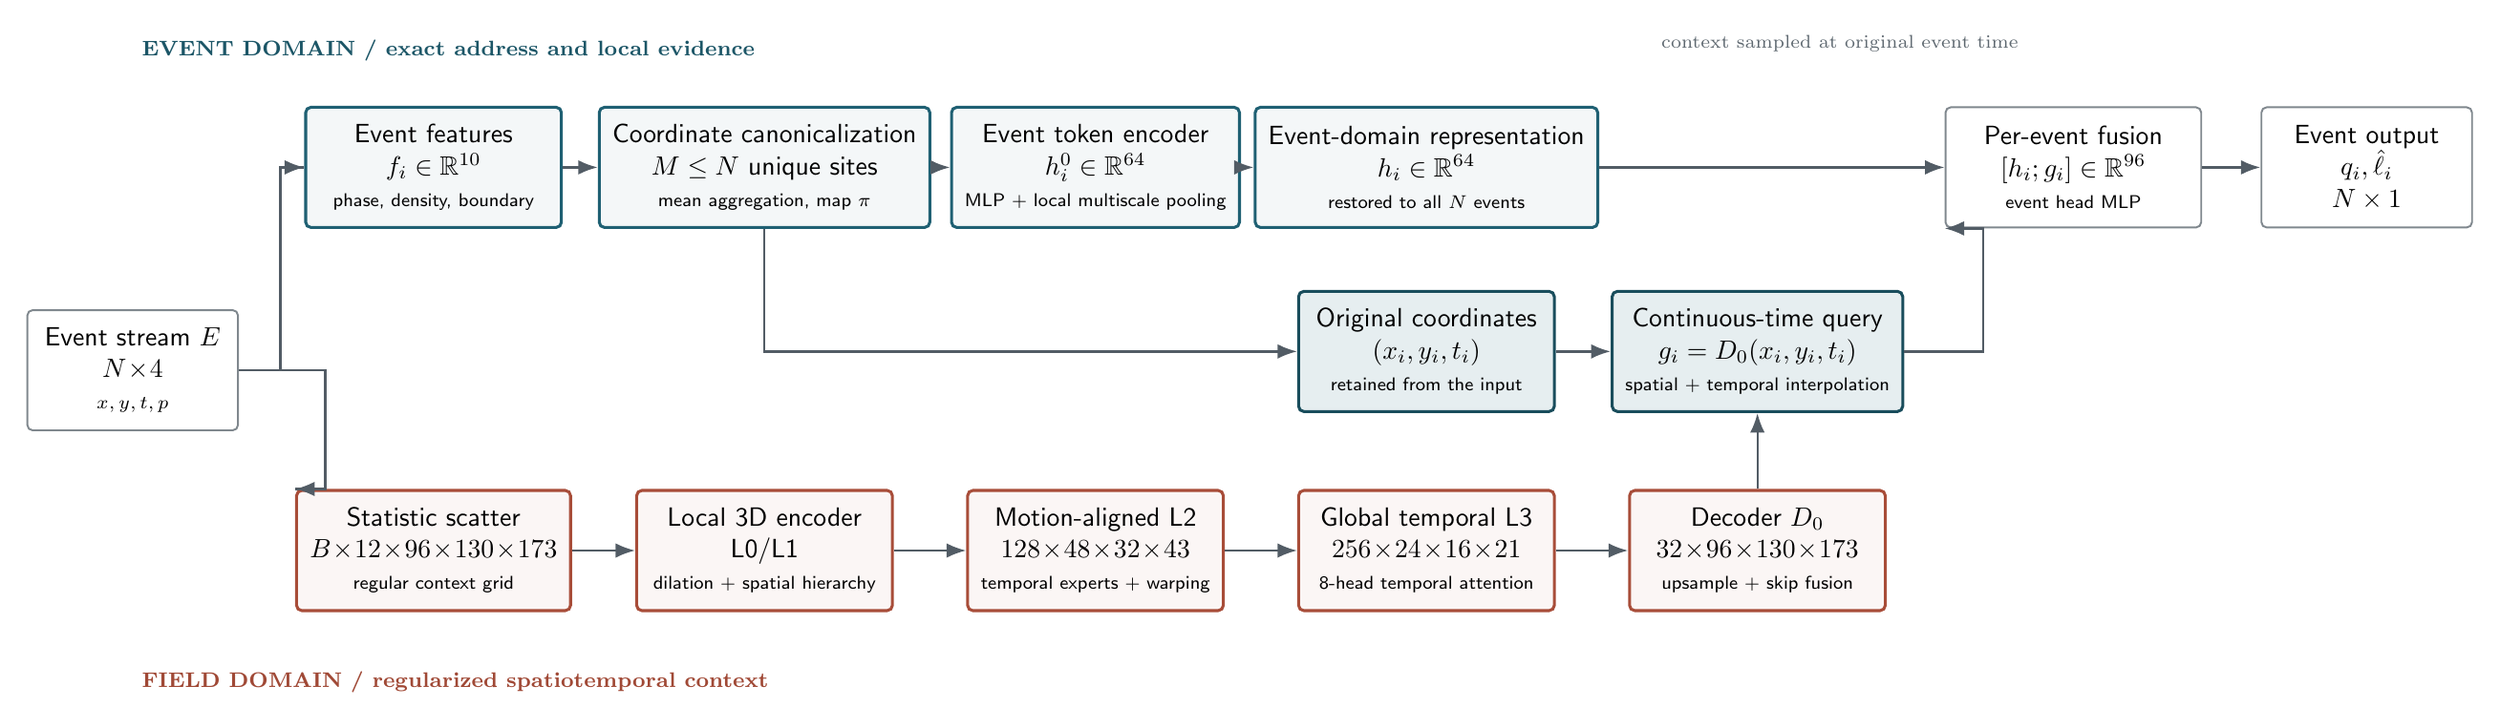
\begin{tikzpicture}[
  font=\sffamily\normalsize, >=Latex,
  box/.style={draw=ink!55, fill=white, line width=.7pt, rounded corners=2pt, minimum width=34mm, minimum height=16mm, align=center, inner sep=5pt},
  event/.style={box,draw=sea,line width=1.1pt,fill=sea!5},
  field/.style={box,draw=rust,line width=1.1pt,fill=rust!5},
  query/.style={box,draw=sea!80!black,line width=1.1pt,fill=sea!11},
  arrow/.style={-{Latex[length=2.6mm]},draw=ink!75,line width=.85pt},
  label/.style={font=\footnotesize\bfseries,color=sea!90!black},
  sub/.style={font=\scriptsize,color=ink!70,align=center}
]
  % Shared input
  \node[box,minimum width=28mm] (src) at (0,0) {Event stream $E$\\$N\!\times\!4$\\{\scriptsize $x,y,t,p$}};

  % Event-domain lane
  \node[event] (feat) at (4.0,2.7) {Event features\\$f_i\in\mathbb R^{10}$\\{\scriptsize phase, density, boundary}};
  \node[event] (canon) at (8.4,2.7) {Coordinate canonicalization\\$M\le N$ unique sites\\{\scriptsize mean aggregation, map $\pi$}};
  \node[event] (token) at (12.8,2.7) {Event token encoder\\$h_i^0\in\mathbb R^{64}$\\{\scriptsize MLP + local multiscale pooling}};
  \node[event] (eventout) at (17.2,2.7) {Event-domain representation\\$h_i\in\mathbb R^{64}$\\{\scriptsize restored to all $N$ events}};

  % Field-domain lane
  \node[field] (scatter) at (4.0,-2.4) {Statistic scatter\\$B\!\times\!12\!\times\!96\!\times\!130\!\times\!173$\\{\scriptsize regular context grid}};
  \node[field] (local) at (8.4,-2.4) {Local 3D encoder\\L0/L1\\{\scriptsize dilation + spatial hierarchy}};
  \node[field] (align) at (12.8,-2.4) {Motion-aligned L2\\$128\!\times\!48\!\times\!32\!\times\!43$\\{\scriptsize temporal experts + warping}};
  \node[field] (global) at (17.2,-2.4) {Global temporal L3\\$256\!\times\!24\!\times\!16\!\times\!21$\\{\scriptsize 8-head temporal attention}};
  \node[field] (decode) at (21.6,-2.4) {Decoder $D_0$\\$32\!\times\!96\!\times\!130\!\times\!173$\\{\scriptsize upsample + skip fusion}};

  % Query and output
  \node[query] (coords) at (17.2,.25) {Original coordinates\\$(x_i,y_i,t_i)$\\{\scriptsize retained from the input}};
  \node[query] (query) at (21.6,.25) {Continuous-time query\\$g_i=D_0(x_i,y_i,t_i)$\\{\scriptsize spatial + temporal interpolation}};
  \node[box] (fusion) at (25.8,2.7) {Per-event fusion\\$[h_i;g_i]\in\mathbb R^{96}$\\{\scriptsize event head MLP}};
  \node[box,minimum width=28mm] (out) at (29.7,2.7) {Event output\\$q_i,\hat\ell_i$\\$N\times1$};

  % Lane labels
  \node[label,anchor=west] at (0,4.25) {EVENT DOMAIN  /  exact address and local evidence};
  \node[label,anchor=west,color=rust!95!black] at (0,-4.15) {FIELD DOMAIN  /  regularized spatiotemporal context};
  % The shared-input relation is represented by the two explicit buses below.
  \node[sub,anchor=west] at (20.2,4.35) {context sampled at original event time};

  % Main arrows: explicit separated buses for the two domains
  \draw[draw=ink!75,line width=.85pt] (src.east) -- ++(.55,0) |- (feat.west);
  \draw[arrow] (src.east) -- ++(.55,0) |- (feat.west);
  \draw[arrow] (feat) -- (canon);
  \draw[arrow] (canon) -- (token);
  \draw[arrow] (token) -- (eventout);
  \draw[draw=ink!75,line width=.85pt] (src.east) -- ++(1.15,0) |- (scatter.north west);
  \draw[arrow] (src.east) -- ++(1.15,0) |- (scatter.north west);
  \draw[arrow] (scatter) -- (local);
  \draw[arrow] (local) -- (align);
  \draw[arrow] (align) -- (global);
  \draw[arrow] (global) -- (decode);
  \draw[arrow] (canon.south) |- (coords.west);
  \draw[arrow] (decode.north) -- (query.south);
  \draw[arrow] (coords.east) -- (query.west);
  \draw[arrow] (eventout) -- (fusion);
  \draw[arrow] (query.east) -- ++(1.05,0) |- (fusion.south west);
  \draw[arrow] (fusion) -- (out);
\end{tikzpicture}
\end{document}
